\documentclass[border=3pt]{standalone}
% Preâmbulo compartilhado pelos diagramas TikZ da aula 14 (SLAM com EIF)
\usepackage[T1]{fontenc}
\usepackage[utf8]{inputenc}
\usepackage{lmodern}
\usepackage{amsmath}
\usepackage{xcolor}
\usepackage{tikz}
\usetikzlibrary{arrows.meta,angles,quotes,decorations.pathmorphing,decorations.pathreplacing,calc,
                positioning,shapes.geometric,shapes.misc,backgrounds,fit,
                math}

% Paleta (mesma dos SVGs originais)
\definecolor{dblue}{HTML}{2A5B8C}
\definecolor{dorange}{HTML}{B3541E}
\definecolor{dgreen}{HTML}{4A7C59}
\definecolor{dred}{HTML}{9C4B4B}
\definecolor{dcream}{HTML}{F4F1EA}
\definecolor{dshade}{HTML}{DDD7C9}

% Função gaussiana (não normalizada por padrão de escala visual)
\pgfmathdeclarefunction{gauss}{3}{%
  \pgfmathparse{1/(#3*sqrt(2*pi))*exp(-((#1-#2)^2)/(2*#3^2))}%
}

% Estilos comuns (prefixo d... para não colidir com chaves internas do pgf)
\tikzset{
  >={Stealth[length=2mm]},
  dguide/.style={gray!55, dashed, line width=0.4pt},
  daxis/.style={gray!60, line width=0.7pt, ->},
  dbody/.style={fill=black!3, draw=black!80, line width=1pt},
  dacc/.style={draw=dblue, line width=1pt},
  dlbl/.style={black!55, font=\small},
  dsub/.style={black!45, font=\footnotesize},
  dstate/.style={circle, draw=black!80, fill=dcream, line width=1pt,
                 minimum size=17mm, font=\large, inner sep=1pt},
  dobs/.style={circle, draw=black!80, fill=dshade, line width=1pt,
               minimum size=14mm, font=\large, inner sep=1pt},
  dbox/.style={rounded corners=2pt, draw=black!80, fill=dcream, line width=1pt,
               align=center, inner sep=6pt},
  dop/.style={circle, draw=black!80, fill=white, line width=1pt,
              minimum size=6mm, inner sep=0pt, font=\small},
  dtrans/.style={->, dblue, line width=1pt},
  dmeas/.style={->, dorange, line width=1pt},
  dcurve/.style={line width=1pt, dblue},
  dcurveb/.style={line width=1.4pt, dorange},
}

\begin{document}
\hyphenpenalty=10000 \exhyphenpenalty=10000 \tolerance=9999 \emergencystretch=3em
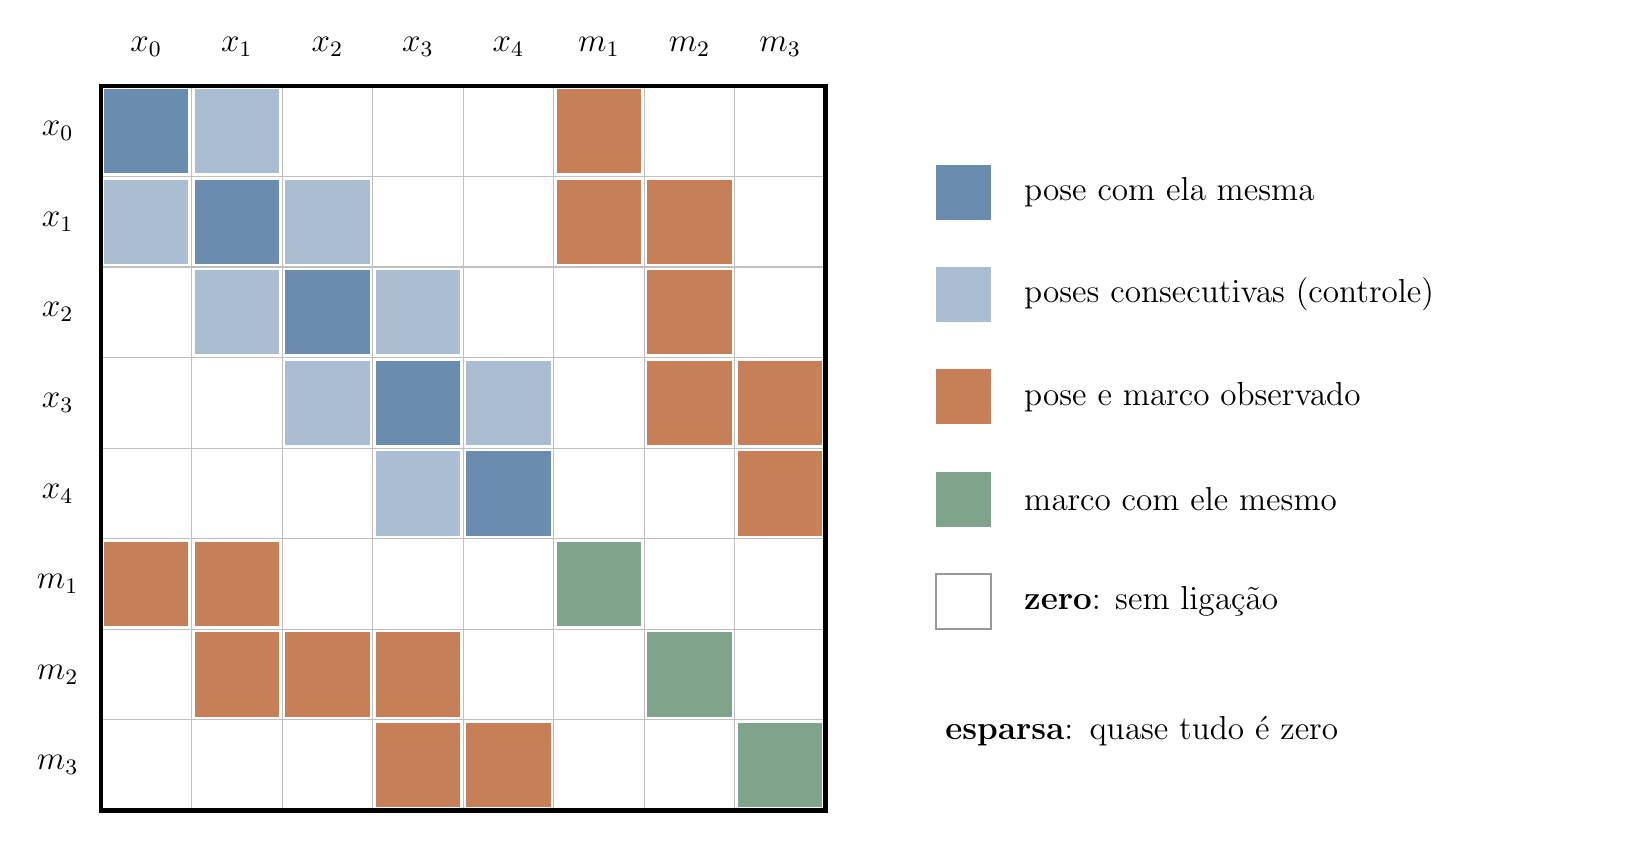
\begin{tikzpicture}[x=1cm,y=1cm]
\def\cw{1.15}
\foreach \i in {0,...,7} {
  \foreach \j in {0,...,7} {\draw[black!25, line width=0.4pt] ({\j*\cw},{-\i*\cw}) rectangle ({(\j+1)*\cw},{-(\i+1)*\cw});}}
% diagonal e vizinhas: poses x0..x4 (indices 0..4)
\foreach \i in {0,...,4} {\fill[dblue!70] ({\i*\cw+0.04},{-\i*\cw-0.04}) rectangle ({(\i+1)*\cw-0.04},{-(\i+1)*\cw+0.04});}
\foreach \i in {0,...,3} {\pgfmathtruncatemacro{\k}{\i+1}
  \fill[dblue!40] ({\k*\cw+0.04},{-\i*\cw-0.04}) rectangle ({(\k+1)*\cw-0.04},{-(\i+1)*\cw+0.04});
  \fill[dblue!40] ({\i*\cw+0.04},{-\k*\cw-0.04}) rectangle ({(\i+1)*\cw-0.04},{-(\k+1)*\cw+0.04});}
% marcos m1,m2,m3 = indices 5,6,7 : diagonal
\foreach \i in {5,6,7} {\fill[dgreen!70] ({\i*\cw+0.04},{-\i*\cw-0.04}) rectangle ({(\i+1)*\cw-0.04},{-(\i+1)*\cw+0.04});}
% pose-marco
\foreach \p/\mm in {0/5,1/5,1/6,2/6,3/6,3/7,4/7} {
  \fill[dorange!75] ({\mm*\cw+0.04},{-\p*\cw-0.04}) rectangle ({(\mm+1)*\cw-0.04},{-(\p+1)*\cw+0.04});
  \fill[dorange!75] ({\p*\cw+0.04},{-\mm*\cw-0.04}) rectangle ({(\p+1)*\cw-0.04},{-(\mm+1)*\cw+0.04});}
\foreach \i/\t in {0/{$x_0$},1/{$x_1$},2/{$x_2$},3/{$x_3$},4/{$x_4$},5/{$m_1$},6/{$m_2$},7/{$m_3$}} {
  \node[font=\large] at ({\i*\cw+0.575},0.5) {\t};
  \node[font=\large] at (-0.55,{-\i*\cw-0.575}) {\t};}
\draw[line width=1.6pt] (0,0) rectangle (9.2,-9.2);
\def\lx{10.6}
\fill[dblue!70] (\lx,-1.0) rectangle (\lx+0.7,-1.7); \node[font=\large, anchor=west] at (\lx+1.0,-1.35) {pose com ela mesma};
\fill[dblue!40] (\lx,-2.3) rectangle (\lx+0.7,-3.0); \node[font=\large, anchor=west] at (\lx+1.0,-2.65) {poses consecutivas (controle)};
\fill[dorange!75] (\lx,-3.6) rectangle (\lx+0.7,-4.3); \node[font=\large, anchor=west] at (\lx+1.0,-3.95) {pose e marco observado};
\fill[dgreen!70] (\lx,-4.9) rectangle (\lx+0.7,-5.6); \node[font=\large, anchor=west] at (\lx+1.0,-5.25) {marco com ele mesmo};
\draw[black!40, line width=0.8pt] (\lx,-6.2) rectangle (\lx+0.7,-6.9); \node[font=\large, anchor=west] at (\lx+1.0,-6.55) {\textbf{zero}: sem ligação};
\node[font=\large, anchor=west, text width=8.2cm] at (\lx,-8.2) {\textbf{esparsa}: quase tudo é zero};
\end{tikzpicture}
\end{document}
